\documentclass[10pt,letterpaper]{article}

% Stable output supports docs:check even when translation uses a temporary directory.
\ifdefined\pdftrailerid
  \pdftrailerid{}
\fi

\usepackage[T1]{fontenc}
\usepackage[utf8]{inputenc}
\usepackage{lmodern}
\usepackage[margin=0.72in]{geometry}
\usepackage{amsmath,amssymb,mathtools}
\usepackage{booktabs,longtable,tabularx,array}
\usepackage[dvipsnames,table]{xcolor}
\usepackage{listings}
\usepackage{tikz}
\usepackage{enumitem}
\usepackage{fancyhdr}
\usepackage{microtype}
\usepackage[hidelinks]{hyperref}
\usepackage{bookmark}
\usepackage{titlesec}

\usetikzlibrary{arrows.meta,calc,positioning}

\definecolor{QpuNavy}{HTML}{0F172A}
\definecolor{QpuBlue}{HTML}{2563EB}
\definecolor{QpuCyan}{HTML}{0891B2}
\definecolor{QpuGreen}{HTML}{047857}
\definecolor{QpuAmber}{HTML}{B45309}
\definecolor{QpuRed}{HTML}{B91C1C}
\definecolor{QpuPaper}{HTML}{F8FAFC}
\definecolor{QpuLine}{HTML}{CBD5E1}
\definecolor{CodeBg}{HTML}{F1F5F9}
\definecolor{CodeComment}{HTML}{64748B}

\providecommand{\QpuDocTitle}{QPU Documentation}
\providecommand{\QpuDocSubtitle}{System Guide}
\providecommand{\QpuDocDescription}{A guide to the QPU circuit system.}
\providecommand{\QpuHeaderTitle}{QPU Documentation}

\hypersetup{
  pdftitle={\QpuDocTitle: \QpuDocSubtitle},
  pdfauthor={Bailey Forbes},
  pdfsubject={QPU protocol syntax, quantum gates, mathematics, and truth tables},
  pdfkeywords={QPU, quantum circuit, protocol, system syntax, truth table}
}

\pagestyle{fancy}
\fancyhf{}
\lhead{\textcolor{QpuNavy}{QPU Circuit Compiler}}
\rhead{\textcolor{QpuNavy}{\QpuHeaderTitle}}
\cfoot{\thepage}
\renewcommand{\headrulewidth}{0.3pt}

\titleformat{\section}{\Large\bfseries\color{QpuNavy}}{\thesection}{0.55em}{}
\titleformat{\subsection}{\large\bfseries\color{QpuBlue}}{\thesubsection}{0.5em}{}
\titleformat{\subsubsection}{\normalsize\bfseries\color{QpuCyan}}{\thesubsubsection}{0.45em}{}
\setlist{nosep,leftmargin=1.5em}
\setlength{\parindent}{0pt}
\setlength{\parskip}{4pt}
\setlength{\tabcolsep}{4pt}
\renewcommand{\arraystretch}{1.15}

\lstdefinelanguage{QPU}{
  morekeywords={
    PARAMS,MAIN-PROCESS,INCREASECYCLE,COMPILEPROCESS,FREE,SET,JOIN,SPLIT,
    CALL,DECLARECHILD,RUNCHILD,REC,TREC,RECUR,EXIT,IF,ELSE,ENDIF,RETURNVALS,ACCEPTVALS,MASTERVAL,SAVE_STATE,
    LOAD_STATE,CREATETOKEN,DELETETOKEN,X,Y,Z,H,S,T,CNOT,CCNOT,CZ,CY,
    SWAP,PHASE,RX,RY,RZ,CPHASE,MEASURE,NOT,AND,NAND,OR,XOR
  },
  sensitive=false,
  morecomment=[l]{\#},
  morecomment=[s]{/*}{*/},
  morestring=[b]"
}
\lstset{
  language=QPU,
  basicstyle=\ttfamily\small,
  keywordstyle=\bfseries\color{QpuBlue},
  commentstyle=\itshape\color{CodeComment},
  backgroundcolor=\color{CodeBg},
  frame=single,
  rulecolor=\color{QpuLine},
  framerule=0.4pt,
  xleftmargin=0.4em,
  framexleftmargin=0.35em,
  columns=fullflexible,
  keepspaces=true,
  showstringspaces=false,
  breaklines=true,
  aboveskip=5pt,
  belowskip=5pt
}

\newcommand{\code}[1]{\texttt{\detokenize{#1}}}
\newcommand{\ket}[1]{\lvert #1\rangle}
\newcommand{\bra}[1]{\langle #1\rvert}
\newcommand{\status}[1]{\textsf{\small #1}}
\newcommand{\implemented}{\textcolor{QpuGreen}{\status{lowered/executed}}}
\newcommand{\acceptedonly}{\textcolor{QpuAmber}{\status{accepted, not executed}}}
\newcommand{\internal}{\textcolor{QpuCyan}{\status{compiler-internal}}}

\newcommand{\GateSegment}[1]{%
\begin{tikzpicture}[baseline=-0.55ex,scale=.78]
  \draw[thick] (0,0)--(3.6,0);
  \node[left] at (0,0) {$\ket{q}$};
  \node[draw=QpuBlue,fill=QpuBlue!8,minimum width=.62cm,minimum height=.55cm,font=\bfseries] at (1.8,0) {#1};
\end{tikzpicture}}

\newcommand{\ControlledSegment}[1]{%
\begin{tikzpicture}[baseline=-0.55ex,scale=.78]
  \draw[thick] (0,.55)--(3.6,.55);
  \draw[thick] (0,-.55)--(3.6,-.55);
  \node[left] at (0,.55) {$\ket{c}$};
  \node[left] at (0,-.55) {$\ket{t}$};
  \fill[QpuNavy] (1.8,.55) circle (.09);
  \draw[thick] (1.8,.55)--(1.8,-.55);
  \node[draw=QpuBlue,fill=QpuBlue!8,circle,inner sep=1.7pt,font=\scriptsize\bfseries] at (1.8,-.55) {#1};
\end{tikzpicture}}

\newcommand{\DoubleControlledSegment}{%
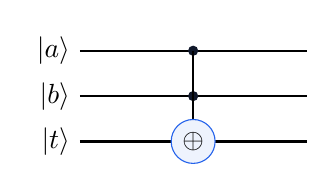
\begin{tikzpicture}[baseline=-0.55ex,scale=.72]
  \foreach \y/\n in {.8/a,0/b,-.8/t} {
    \draw[thick] (0,\y)--(4,\y);
    \node[left] at (0,\y) {$\ket{\n}$};
  }
  \fill[QpuNavy] (2,.8) circle (.09);
  \fill[QpuNavy] (2,0) circle (.09);
  \draw[thick] (2,.8)--(2,-.8);
  \node[draw=QpuBlue,fill=QpuBlue!8,circle,inner sep=2pt,font=\bfseries] at (2,-.8) {$\oplus$};
\end{tikzpicture}}

\newcommand{\SwapSegment}{%
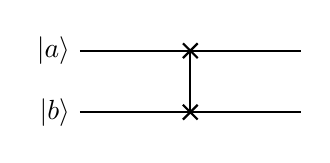
\begin{tikzpicture}[baseline=-0.55ex,scale=.78]
  \draw[thick] (0,.5)--(3.6,.5);
  \draw[thick] (0,-.5)--(3.6,-.5);
  \node[left] at (0,.5) {$\ket{a}$};
  \node[left] at (0,-.5) {$\ket{b}$};
  \draw[thick] (1.68,.38)--(1.92,.62) (1.68,.62)--(1.92,.38);
  \draw[thick] (1.68,-.38)--(1.92,-.62) (1.68,-.62)--(1.92,-.38);
  \draw[thick] (1.8,.5)--(1.8,-.5);
\end{tikzpicture}}

\newcommand{\QpuMeter}[2]{%
  \begin{scope}[shift={(#1,#2)}]
    \draw[QpuBlue,thick] (-0.28,-0.22) rectangle (0.28,0.28);
    \draw[QpuBlue,thick] (-0.18,-0.02) arc (180:0:0.18);
    \draw[QpuBlue,thick] (0,-0.02) -- (0.14,0.16);
    \fill[QpuBlue] (0,-0.02) circle (0.035);
  \end{scope}}
\newcommand{\MeasureSegment}{%
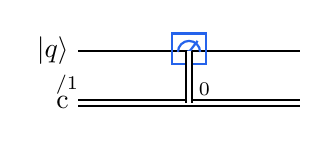
\begin{tikzpicture}[baseline=-0.55ex,scale=.78]
  \draw[thick] (0,0)--(3.6,0);
  \node[left] at (0,0) {$\ket{q}$};
  \QpuMeter{1.8}{0}
  \draw[double distance=1.4pt,thick] (0,-.85)--(3.6,-.85);
  \node[left] at (0,-.85) {c};
  \node[left,font=\scriptsize] at (0.15,-.55) {/1};
  \draw[double distance=1.4pt,thick] (1.8,0)--(1.8,-.85);
  \node[right,font=\scriptsize] at (1.8,-.62) {0};
\end{tikzpicture}}

% The hypertarget gives each gate a stable PDF named destination (gate-CNOT,
% gate-H, ...) that the workbench links to with #nameddest=.
\newcommand{\GateHeading}[3]{%
\subsection{#1 (\code{#2})}\hypertarget{gate-#2}{}
\begin{center}#3\end{center}}

% Short framed callouts. The body is boxed, so it cannot contain lstlisting
% and should stay short enough to fit on one page.
\newsavebox{\QpuCalloutBox}
\newenvironment{QpuCallout}[2]{%
  \def\QpuCalloutColor{#1}%
  \setlength{\fboxrule}{0.6pt}%
  \par\smallskip\noindent
  \begin{lrbox}{\QpuCalloutBox}%
  \begin{minipage}{\dimexpr\linewidth-2\fboxsep-2\fboxrule\relax}%
  \setlength{\parskip}{3pt}%
  {\bfseries\color{#1}#2}\par
}{%
  \end{minipage}%
  \end{lrbox}%
  \fcolorbox{\QpuCalloutColor}{\QpuCalloutColor!6}{\usebox{\QpuCalloutBox}}%
  \par\smallskip
}
\newenvironment{beginnerbox}[1][Beginner note]{\begin{QpuCallout}{QpuGreen}{#1}}{\end{QpuCallout}}
\newenvironment{trybox}[1][Try it in the Circuit builder]{\begin{QpuCallout}{QpuBlue}{#1}}{\end{QpuCallout}}
\newenvironment{cautionbox}[1][Watch out]{\begin{QpuCallout}{QpuAmber}{#1}}{\end{QpuCallout}}

% Workbench selectors on the left, the circuit diagram they produce on the
% right. #1 is the gate name shown in the Gate selector and on the target.
\newcommand{\WorkbenchControlMap}[1]{%
\begin{tikzpicture}[font=\small,>={Latex[length=2mm]}]
  \tikzset{ui/.style={draw=##1,rounded corners=2pt,anchor=west,minimum width=3.9cm,minimum height=.55cm,inner sep=3pt}}
  \node[ui=QpuLine,fill=CodeBg] at (0,1.75) {\textsf{Gate:} \textbf{#1}};
  \node[ui=QpuBlue,fill=QpuBlue!8] (a) at (0,.95) {\textsf{Control A:} \textbf{q0}};
  \node[ui=QpuBlue,fill=QpuBlue!8] (b) at (0,.15) {\textsf{Control B:} \textbf{q1}};
  \node[ui=QpuRed,fill=QpuRed!6] (t) at (0,-.65) {\textsf{Target particle:} \textbf{q2}};
  \node[font=\scriptsize\bfseries,color=QpuNavy,anchor=west] at (0,2.45) {Interactive workbench};
  \node[font=\scriptsize\bfseries,color=QpuNavy] at (7.4,2.45) {Circuit canvas};
  \foreach \y/\q in {.95/q0,.15/q1,-.65/q2} {
    \draw[thick] (5.6,\y)--(9.2,\y);
    \node[left,font=\scriptsize] at (5.6,\y) {\q};
  }
  \draw[->,dashed,QpuBlue] (a.east)--(5.05,.95);
  \draw[->,dashed,QpuBlue] (b.east)--(5.05,.15);
  \draw[->,dashed,QpuRed] (t.east)--(5.05,-.65);
  \fill[QpuNavy] (7.4,.95) circle (.09);
  \fill[QpuNavy] (7.4,.15) circle (.09);
  \draw[thick] (7.4,.95)--(7.4,-.65);
  \node[draw=QpuRed,fill=QpuRed!6,circle,inner sep=1.5pt,font=\bfseries] at (7.4,-.65) {$\oplus$};
  \node[anchor=west,font=\scriptsize] at (9.3,.95) {$A$: read, left unchanged};
  \node[anchor=west,font=\scriptsize] at (9.3,.15) {$B$: read, left unchanged};
  \node[anchor=west,font=\scriptsize] at (9.3,-.65) {$t' = t\oplus(A\land B)$: written};
\end{tikzpicture}}

\newcommand{\QpuTitlePage}{%
\begin{titlepage}
\pagecolor{QpuPaper}
\centering
\vspace*{1.15in}
{\Huge\bfseries\color{QpuNavy} \QpuDocTitle\par}
\vspace{0.2in}
{\LARGE\color{QpuBlue} \QpuDocSubtitle\par}
\vspace{0.55in}
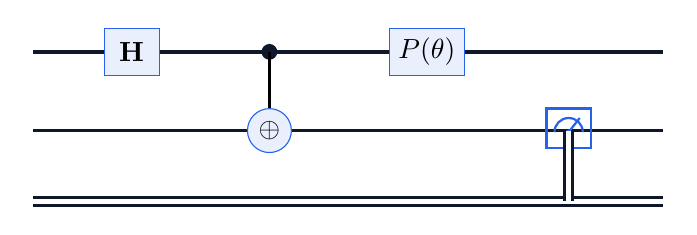
\begin{tikzpicture}
  \draw[very thick,QpuNavy] (0,1)--(8,1);
  \draw[very thick,QpuNavy] (0,0)--(8,0);
  \draw[double distance=1.6pt,very thick,QpuNavy] (0,-.9)--(8,-.9);
  \node[draw=QpuBlue,fill=QpuBlue!10,minimum width=.7cm,minimum height=.6cm,font=\bfseries] at (1.25,1) {H};
  \fill[QpuNavy] (3,1) circle (.1);
  \draw[very thick] (3,1)--(3,0);
  \node[draw=QpuBlue,fill=QpuBlue!10,circle,inner sep=2pt] at (3,0) {$\oplus$};
  \node[draw=QpuBlue,fill=QpuBlue!10,minimum width=.8cm,minimum height=.6cm,font=\bfseries] at (5,1) {$P(\theta)$};
  \QpuMeter{6.8}{0}
  \draw[double distance=1.6pt,very thick,QpuNavy] (6.8,0)--(6.8,-.9);
\end{tikzpicture}
\vfill
{\large Bailey Forbes\par}
{\large September 13, 2026\par}
\vspace{0.35in}
\begin{minipage}{0.82\textwidth}
\small\color{QpuNavy}
\QpuDocDescription
\end{minipage}
\vfill
\end{titlepage}
\nopagecolor
}

% Widen the TOC number column so two-digit subsections (13.10) keep a gap before the title.
\makeatletter
\renewcommand*\l@subsection{\@dottedtocline{2}{1.5em}{2.8em}}
\renewcommand*\l@subsubsection{\@dottedtocline{3}{4.3em}{3.6em}}
\makeatother

\newcommand{\QpuContents}{%
\pagenumbering{roman}
\tableofcontents
\clearpage
\pagenumbering{arabic}
}
